%!TEX root = ../report.tex
\section{Isolines}
\label{sec:isolines}
An isoline shows all points of a scalar dataset's domain where the scalar is equal to a certain value.
Many people are familiar with isolines, because they are used often in weather forecasts, and terrain height maps.

\subsection{Marching squares}
An efficient algorithm to construct these isolines is called the \textit{Marching squares}\cite{maple2003geometric} algorithm, which we have implemented in our application.
The general idea of the algorithm is to loop over all cells and mark for all vertices if the value at that vertex is above or below the isoline value.
After marking the four vertices, \(2^4=16\) different cases can occur, where each case can be coded individually.
The cases determine through which sides of the cell a line should be drawn, if any.
At each side where a line should be drawn, we interpolate to determine the exact position where the cell side has the same value as the isoline value.
Since the starting location of a line is the end location of another line from a different cell, a reasonably smooth, closed curve is created.

\(16\) cases seems like a lot, but we have exploited the symmetry of the geometry to reduce it to only \(8\) cases where something has to happen.
For example, two cases that can be handled identically are shown in Figure~\ref{fig:iso_example}.
\begin{figure}[htb]
    \centering
    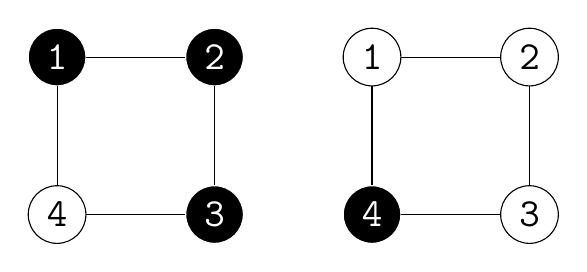
\begin{tikzpicture}[node distance=2cm,
        low node/.style={black,circle,fill=white,draw,font=\ttfamily\Large},
        high node/.style={white,circle,fill=black,draw,font=\ttfamily\Large}]

        \node[high node] (1)              {1};
        \node[high node] (2) [right of=1] {2};
        \node[high node] (3) [below of=2] {3};
        \node[low node]  (4) [left of=3]  {4};

        \node[low node] (5) [right of=2] {1};
        \node[low node] (6) [right of=5] {2};
        \node[low node] (7) [below of=6] {3};
        \node[high node]  (8) [left of=7]  {4};

        \path
            (1) edge [-] node {} (2)
            (2) edge [-] node {} (3)
            (3) edge [-] node {} (4)
            (4) edge [-] node {} (1);
        \path
            (5) edge [-] node {} (6)
            (6) edge [-] node {} (7)
            (7) edge [-] node {} (8)
            (8) edge [-] node {} (5);
    \end{tikzpicture}
    \caption{Two cases that can be handled in the same manner, namely, by drawing the isoline between the edges \((1)-(4)\) and \((3)-(4)\). A black node indicates a value higher than the isoline value, and a white node indicates a value lower than the isoline value.}
    \label{fig:iso_example}
\end{figure}

\subsection{Interaction}
The user of the application is able to set the upper and lower limit of the isoline values, and the number of isolines that are desired.
The application will space the isoline values linearly between the upper and lower limit.

The user is also able to change the colormap that is used to draw the isolines.

\begin{figure}[htb]
  \centering
  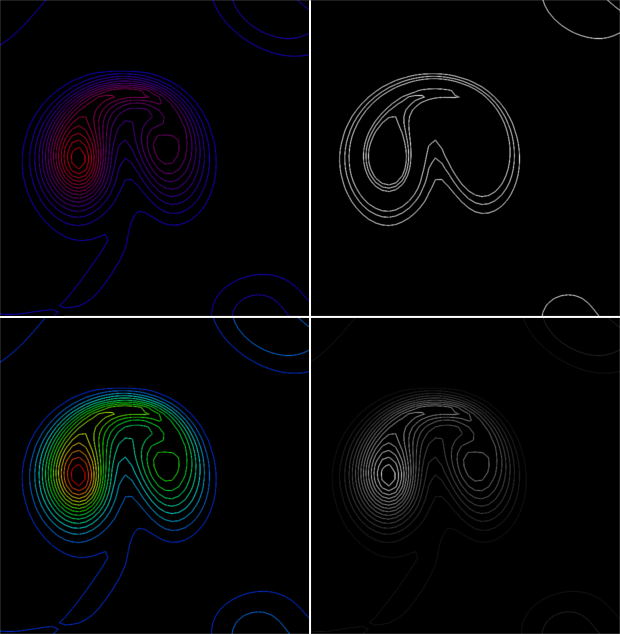
\includegraphics[width=\linewidth]{./content/pictures/isolines.png}
  \caption{Multiple screenshots of the same isolines, drawn with different color maps. It can be seen that the zebra color map (upper right) is not very appropriate for isolines, since some isolines are drawn in black, and so they are not visible since the background is also black.}
\end{figure}
\clearpage